\documentclass{article}

\usepackage[brazil]{babel}
\usepackage[utf8]{inputenc}
%\UseRawInputEncoding
\usepackage[T1]{fontenc}
\usepackage{Sweave}
\usepackage{animate}
\usepackage{amsbsy}
\usepackage{amsfonts}
\usepackage{amsmath}
\usepackage{amssymb}
\usepackage{amsthm}
\usepackage[toc,page,title,titletoc]{appendix}
\usepackage[fixlanguage]{babelbib}
%\usepackage[pdftex]{color}
\usepackage{dsfont}
\usepackage{esvect}
\usepackage[labelfont=bf]{caption}
\usepackage{float}
\usepackage[Glenn]{fncychap}%Sonny %Conny %Lenny %Glenn %Renje %Bjarne %Bjornstrup
%\usepackage{geometry, calc, color, setspace}%
%\geometry{a4paper, headsep=1.0cm, footskip=1cm, lmargin=3cm, rmargin=2cm, tmargin=3cm, bmargin=2cm}
\usepackage{graphicx}
\usepackage{indentfirst}%Para indentar os parágrafos automáticamente
\usepackage{lipsum}
\usepackage{longtable}
\usepackage{mathtools}
\usepackage{listings}%Inserir codigo do R no latex
\usepackage{multirow}
\usepackage{multicol}
\usepackage{ifthen}
\newboolean{firstanswerofthechapter}  
\usepackage{natbib}
\bibliographystyle{abbrvnat3}
\usepackage[figuresright]{rotating}
\usepackage{spalign}
%\usepackage{pgfpages}
\usepackage{pgfplots}
\usepackage{tikz}
\pgfplotsset{compat=1.15}
\usepackage{mathrsfs}
\usetikzlibrary{arrows}
\usepackage{tasks}
\usepackage{color, colortbl}
\usepackage{xcolor}
\colorlet{lightcyan}{cyan!40!white}
\usepackage{chngcntr}
\usepackage{stackengine}
\usepackage{ragged2e}%para justificar o texto dentro de algum ambiente
\definecolor{Gray}{gray}{0.9}
\definecolor{LightCyan}{rgb}{0.88,1,1}

\usepackage[all]{xy}
\usepackage{hyperref,bookmark}
\hypersetup{
  colorlinks=true,
  linkcolor=blue,
  citecolor=red,
  filecolor=blue,
  urlcolor=blue,
}
\newlength{\longestlabel}
\settowidth{\longestlabel}{\bfseries viii.}

\setcounter{secnumdepth}{0} \setlength{\topmargin}{0cm}
\setlength{\headsep}{-0.3cm} \setlength{\textwidth}{17.5cm}
\setlength{\textheight}{23cm} \setlength{\oddsidemargin}{-0.8cm}
\setlength{\evensidemargin}{0cm} \setlength{\footskip}{-1.5cm}

\usepackage[lastexercise,answerdelayed]{exercise}
\renewcommand{\ExerciseName}{Exercícios}
\renewcommand{\ExerciseHeader}{\noindent\def\stackalignment{l}% code from https://tex.stackexchange.com/a/195118/101651
    \stackunder[0pt]{\colorbox{cyan}{\textcolor{white}{\textbf{\large\ExerciseName}}}}{\textcolor{lightcyan}{\rule{\linewidth}{2pt}}}\medskip}
    
% Partial code taken from http://mirrors.ctan.org/macros/latex/contrib/exercise/exercise.dtx
\newenvironment{ManualExercise}
  {\begin{list}{}{\leftmargin \QuestionIndent
    \partopsep0pt \parsep\parskip \topsep\QuestionBefore
    \itemsep\QuestionBefore \labelwidth2em
    \labelsep.33em
    \usecounter{Question}}}
  {\end{list}}    

\begin{document}

\Sconcordance{concordance:TH.tex:TH.Rnw:%
1 141 1 1 19 1 2 5 1 1 2 6 0 1 1 5 0 1 1 5 0 1 1 1 4 3 0 12 1 1 2 6 0 1 %
2 6 0 1 2 6 0 1 2 7 0 1 2 16 1 1 19 1 2 5 1 1 2 6 0 1 1 5 0 1 1 5 0 1 1 %
1 4 3 0 12 1 1 2 6 0 1 2 6 0 1 2 6 0 1 2 7 0 1 2 16 1 1 25 1 2 5 1 1 2 %
1 0 9 1 1 4 3 0 12 1 1 2 6 0 1 2 6 0 1 2 6 0 1 2 7 0 1 2 15 1 1 37 1 2 %
5 1 1 2 6 0 1 1 5 0 1 1 5 0 1 1 5 0 1 1 5 0 1 1 5 0 1 1 5 0 1 1 5 0 1 1 %
5 0 1 1 5 0 1 1 1 4 3 0 1 4 3 0 19 1 1 2 6 0 1 2 6 0 1 2 6 0 1 2 7 0 1 %
2 15 1 1 34 1 2 5 1 1 2 6 0 1 1 5 0 1 1 5 0 1 1 5 0 1 1 5 0 1 1 5 0 1 1 %
5 0 1 1 5 0 1 1 1 4 3 0 1 5 3 0 17 1 1 2 6 0 1 2 6 0 1 2 6 0 1 2 7 0 1 %
2 15 1 1 23 1 2 6 1 1 2 6 0 1 1 5 0 1 1 5 0 1 1 5 0 1 1 5 0 1 1 5 0 1 1 %
5 0 1 1 1 4 3 0 12 1 1 2 6 0 1 2 6 0 1 2 6 0 1 2 7 0 1 2 2 1 1 4 8 0 1 %
1 5 0 1 1 5 0 1 1 5 0 1 1 5 0 1 1 5 0 1 1 5 0 1 1 5 0 2 1 1 2 6 0 1 2 7 %
0 1 2 2 1 1 4 8 0 1 1 5 0 1 1 5 0 1 1 5 0 1 1 5 0 1 1 5 0 1 1 5 0 1 1 5 %
0 1 1 5 0 2 1 1 2 6 0 1 2 7 0 1 2 8 1 1 4 8 0 1 1 5 0 1 1 5 0 1 1 5 0 1 %
1 5 0 1 1 5 0 1 1 5 0 1 1 5 0 1 1 5 0 1 1 5 0 2 1 1 2 6 0 1 2 6 0 1 3 7 %
0 1 1 5 0 1 1 5 0 1 1 5 0 3 1 5 0 1 1 5 0 1 1 5 0 1 1 5 0 2 1 1 2 6 0 1 %
2 7 0 1 2 8 1 1 4 8 0 1 1 5 0 1 1 5 0 1 1 5 0 1 1 5 0 1 1 5 0 1 1 5 0 1 %
1 5 0 1 1 5 0 1 1 5 0 1 1 5 0 1 1 5 0 1 1 5 0 1 1 14 0 2 1 1 2 6 0 1 2 %
6 0 1 3 7 0 1 1 5 0 1 2 6 0 1 1 5 0 1 1 5 0 1 1 5 0 1 1 5 0 1 1 14 0 2 %
1 1 2 6 0 1 2 7 0 1 2 17 1 1 3 8 0 1 2 7 0 1 3 8 0 1 1 5 0 1 1 5 0 1 1 %
5 0 1 1 5 0 1 1 5 0 2 1 5 0 1 1 5 0 1 1 5 0 1 1 14 0 2 1 1 2 6 0 1 2 7 %
0 1 2 3 1}


\vspace*{-2cm}

\begin{center}
\begin{minipage}[s]{2cm}
\hspace{-1.3cm}
\includegraphics[scale=1.0]{Figuras/brasaoufv.eps}
\end{minipage}
\begin{minipage}[s]{13cm}
{\begin{center} {\sc \Large Universidade Federal de Vi\c{c}osa}\\
{\sc \large Instituto de Ci\^encias Exatas e Tecnológicas}\\
{\sc \large Campus UFV - Florestal}\\
\end{center}}
\end{minipage}\begin{minipage}[s]{2 cm}
%\includegraphics[width=2 cm]{logoimecc.eps}
\end{minipage}
\end{center}

\vspace{-0.3cm}

%\hline \hline \noindent

%%%%%%%%%%%%%%%%%%%%%%%%%%%%%%%%%%%%%%%%%%%%%%%%%%%%%%%%%%%%%%%%%%%%%%%%%%%

\medskip

\begin{center}

\underline{\underline{{\large{\sc Soluções da Lista de Testes de Hipóteses}}}}

\bigskip

{\large {\bf Prof. Fernando Bastos}}
%\bigskip
%
%%{\sc Data: $19/06/2018$}
\end{center}


\begin{Exercise}
\begin{ManualExercise} 
\item[9.~]O fabricante de certa marca de suco informa que as embalagens de seu produto têm em média 500 ml, com desvio padrão igual a 10 ml. Tendo sido encontradas no mercado algumas embalagens com menos de 500 ml, suspeita-se que a informação do fabricante seja falsa. Para verificar se isto ocorre, um fiscal analisa uma amostra de 200 embalagens escolhidas aleatoriamente no mercado e constata que as mesmas contêm em média 498 ml. Considerando-se um nível de significância de $5\%,$ pode-se afirmar que o fabricante está mentindo? Calcule o valor da prova para esta amostra.

\begin{align*}
H_{0}: \mu&=500ml \\ 
H_{1}: \mu&<500ml\quad \textrm{(unilateral)}
\end{align*}

Dados:

$n=200;\quad \bar{x}=498ml;\quad \sigma=10ml;\quad \alpha=5\% \rightarrow z_{t}=-1,64$

$$z_{cal}=\dfrac{\bar{x}-\mu_{0}}{\dfrac{\sigma}{\sqrt{n}}}=\dfrac{498-500}{10/\sqrt{200}}=-2.83$$
$$p-valor=0.002338867$$
\begin{center}
\setkeys{Gin}{width=0.5\linewidth}
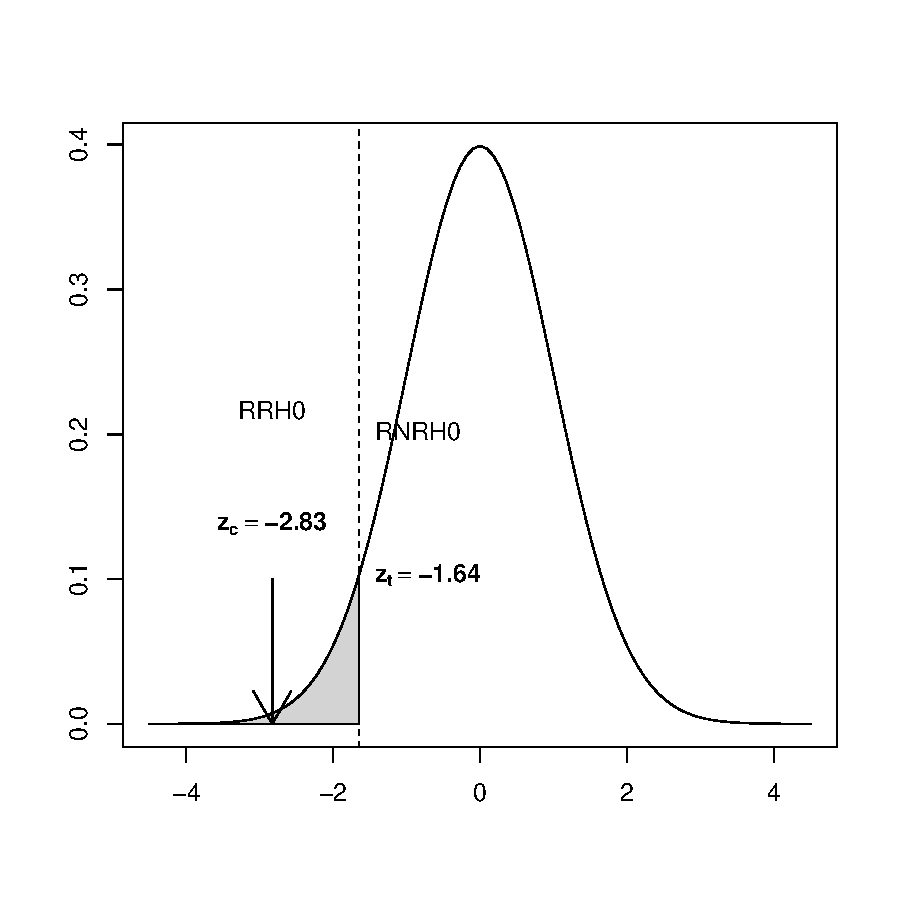
\includegraphics{TH-001}
\end{center}

Decisão: Como $|z_{cal}|>|z_{tab}|$ rejeita-se $H_{0}$ ao nível $\alpha=5\%$ de significância.

Comandos em R para soluções:

\begin{Schunk}
\begin{Sinput}
> (zt <- qnorm(0.05))
\end{Sinput}
\begin{Soutput}
[1] -1.644854
\end{Soutput}
\begin{Sinput}
> (zc <- (498-500)/(10/sqrt(200)))
\end{Sinput}
\begin{Soutput}
[1] -2.828427
\end{Soutput}
\begin{Sinput}
> (pvalor <- pnorm(zc))
\end{Sinput}
\begin{Soutput}
[1] 0.002338867
\end{Soutput}
\begin{Sinput}
> curve(dnorm(x), from=-4.5, to=4.5, xlab="", ylab="")
> polygon(cbind(c(zt,seq(zt,-4.5, l=100),-4.5), 
+               c(0, dnorm(seq(zt, -4.5, l=100)), 
+                 dnorm(-4.5))), 
+         col="lightgray")
> abline(v=zt, lty=2)
> arrows(zc, 0.1, zc, 0)
> zt <- format(zt,digits = 3)
> Zt <- bquote(bold(z[t] == .(zt)))
> zc <- format(zc,digits = 3)
> Zc <- bquote(bold(z[c] == .(zc)))
> text(zt, 0.1, Zt, pos=4)
> text(zt, 0.2, "RNRH0", pos=4)
> text(zc, 0.12, Zc, pos=3)
> text(zc, 0.2, "RRH0", pos=3)
> RR <- "Rejeita-se H0 ao nível de 5% de significância"
> RN <- "Não rejeita-se H0 ao nível de 5% de significância"
> ##Resultado
> ifelse(zc>zt,RR,RN)
\end{Sinput}
\begin{Soutput}
[1] "Rejeita-se H0 ao nível de 5% de significância"
\end{Soutput}
\begin{Sinput}
> ##Ou, equivalentemente:
> ifelse(pvalor > 0.05, RN, RR)
\end{Sinput}
\begin{Soutput}
[1] "Rejeita-se H0 ao nível de 5% de significância"
\end{Soutput}
\begin{Sinput}
> ## estimativa pontual
> (mu.est <- 498)
\end{Sinput}
\begin{Soutput}
[1] 498
\end{Soutput}
\begin{Sinput}
> ## estimativa intervalar (95%)
> (IC.mu <- mu.est + qnorm(c(0.025, 0.975)) * 10/sqrt(200))
\end{Sinput}
\begin{Soutput}
[1] 496.6141 499.3859
\end{Soutput}
\end{Schunk}


\item[10.~]A duração das lâmpadas produzidas por certo fabricante tem distribuição normal com média igual a 1200 horas e desvio padrão igual a 300 horas. O fabricante introduz um novo processo na produção das lâmpadas. Para verificar se o novo processo produz lâmpadas de maior duração, o fabricante observa 100 lâmpadas produzidas pelo novo processo e constata que as mesmas duram em média 1265 horas. Admitindo-se um nível de significância de $5\%,$ pode-se concluir que o novo processo produz lâmpadas com maior duração?

\begin{align*}
H_{0}: \mu&=1200h \\ 
H_{1}: \mu&>1200h\quad \textrm{(unilateral)}
\end{align*}

Dados:

$n=100;\quad \bar{x}=1265h;\quad \sigma=300h;\quad \alpha=5\% \rightarrow z_{t}=1,64$

$$z_{cal}=\dfrac{\bar{x}-\mu_{0}}{\dfrac{\sigma}{\sqrt{n}}}=\dfrac{1265-1200}{300/\sqrt{100}}=2,17$$
$$p-valor=0.01513014$$
\begin{center}
\setkeys{Gin}{width=0.5\linewidth}
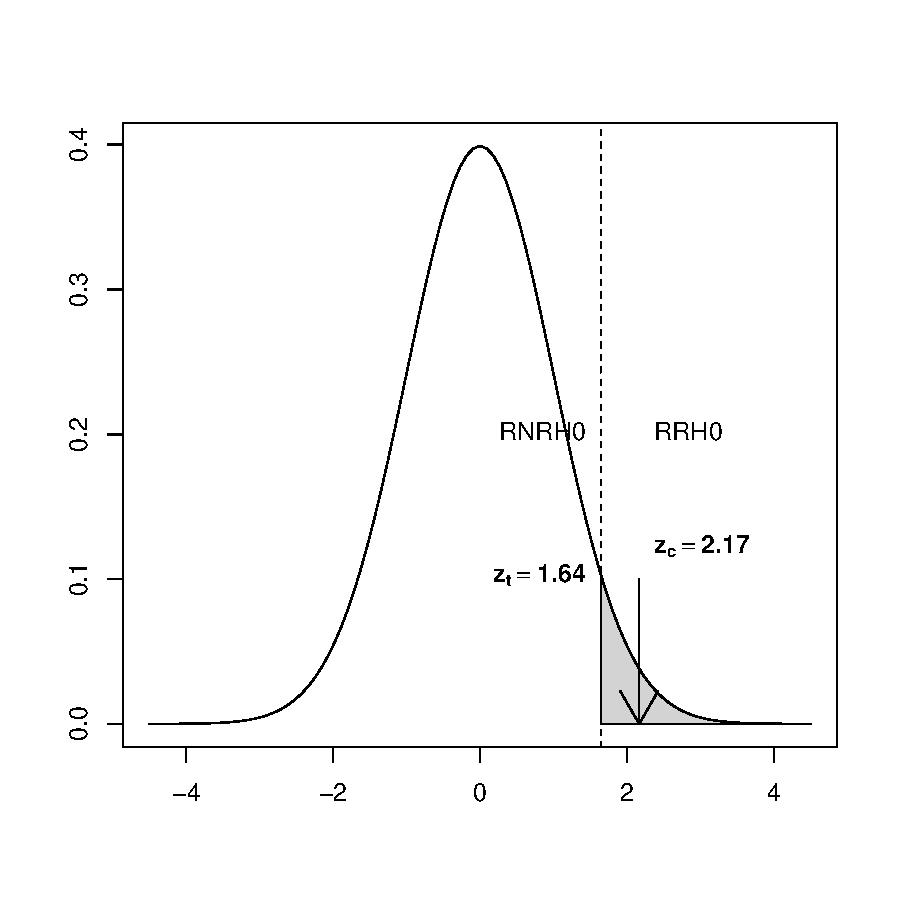
\includegraphics{TH-003}
\end{center}

Decisão: Como $|z_{cal}|>|z_{tab}|$ rejeita-se $H_{0}$ ao nível $\alpha=5\%$ de significância.

Comandos em R para soluções:

\begin{Schunk}
\begin{Sinput}
> (zt <- qnorm(0.95))
\end{Sinput}
\begin{Soutput}
[1] 1.644854
\end{Soutput}
\begin{Sinput}
> (zc <- (1265-1200)/(300/sqrt(100)))
\end{Sinput}
\begin{Soutput}
[1] 2.166667
\end{Soutput}
\begin{Sinput}
> (pvalor <- 1-pnorm(zc))
\end{Sinput}
\begin{Soutput}
[1] 0.01513014
\end{Soutput}
\begin{Sinput}
> curve(dnorm(x), from=-4.5, to=4.5, xlab="", ylab="")
> polygon(cbind(c(zt,seq(zt,4.5, l=100),4.5), 
+               c(0, dnorm(seq(zt, 4.5, l=100)), 
+                 dnorm(4.5))), 
+         col="lightgray")
> abline(v=zt, lty=2)
> arrows(zc, 0.1, zc, 0)
> zt <- format(zt,digits = 3)
> Zt <- bquote(bold(z[t] == .(zt)))
> zc <- format(zc,digits = 3)
> Zc <- bquote(bold(z[c] == .(zc)))
> text(zt, 0.1, Zt, pos=2)
> text(zt, 0.2, "RNRH0", pos=2)
> text(zc, 0.12, Zc, pos=4)
> text(zc, 0.2, "RRH0", pos=4)
> RR <- "Rejeita-se H0 ao nível de 5% de significância"
> RN <- "Não rejeita-se H0 ao nível de 5% de significância"
> ##Resultado
> ifelse(zc>zt,RR,RN)
\end{Sinput}
\begin{Soutput}
[1] "Rejeita-se H0 ao nível de 5% de significância"
\end{Soutput}
\begin{Sinput}
> ##Ou, equivalentemente:
> ifelse(pvalor > 0.05, RN, RR)
\end{Sinput}
\begin{Soutput}
[1] "Rejeita-se H0 ao nível de 5% de significância"
\end{Soutput}
\begin{Sinput}
> ## estimativa pontual
> (mu.est <- 1265)
\end{Sinput}
\begin{Soutput}
[1] 1265
\end{Soutput}
\begin{Sinput}
> ## estimativa intervalar (95%)
> (IC.mu <- mu.est + qnorm(c(0.025, 0.975)) * 300/sqrt(100))
\end{Sinput}
\begin{Soutput}
[1] 1206.201 1323.799
\end{Soutput}
\end{Schunk}

\item[11.~]O custo de produção de certo artigo numa localidade tem distribuição normal com média igual a $R\$42,00.$ Desenvolve-se uma política de redução de custos na empresa para melhorar a competitividade do referido produto no mercado. Observando-se os custos de 10 unidades deste produto, obtiveram-se os seguintes valores: 
$34, 41, 36, 41, 29, 32, 38, 35, 33 e 30.$ Admitindo-se um nível de significância de $5\%,$ pode-se afirmar que o custo do produto considerado diminuiu? 

\begin{align*}
H_{0}: \mu&=R\$42,00 \\
H_{1}: \mu&<R\$42,00\quad \textrm{(unilateral)}
\end{align*}

Dados:

$n=10;\quad \bar{x}=34,9;\quad S=4,17;\quad \alpha=5\% \rightarrow t_{t}=-1.83$

$$t_{cal}=\dfrac{\bar{x}-\mu_{0}}{\dfrac{S}{\sqrt{n}}}=\dfrac{34,9-42}{4,17/\sqrt{10}}=-5,38$$
$$p-valor=0.0002210237$$
\begin{center}
\setkeys{Gin}{width=0.5\linewidth}
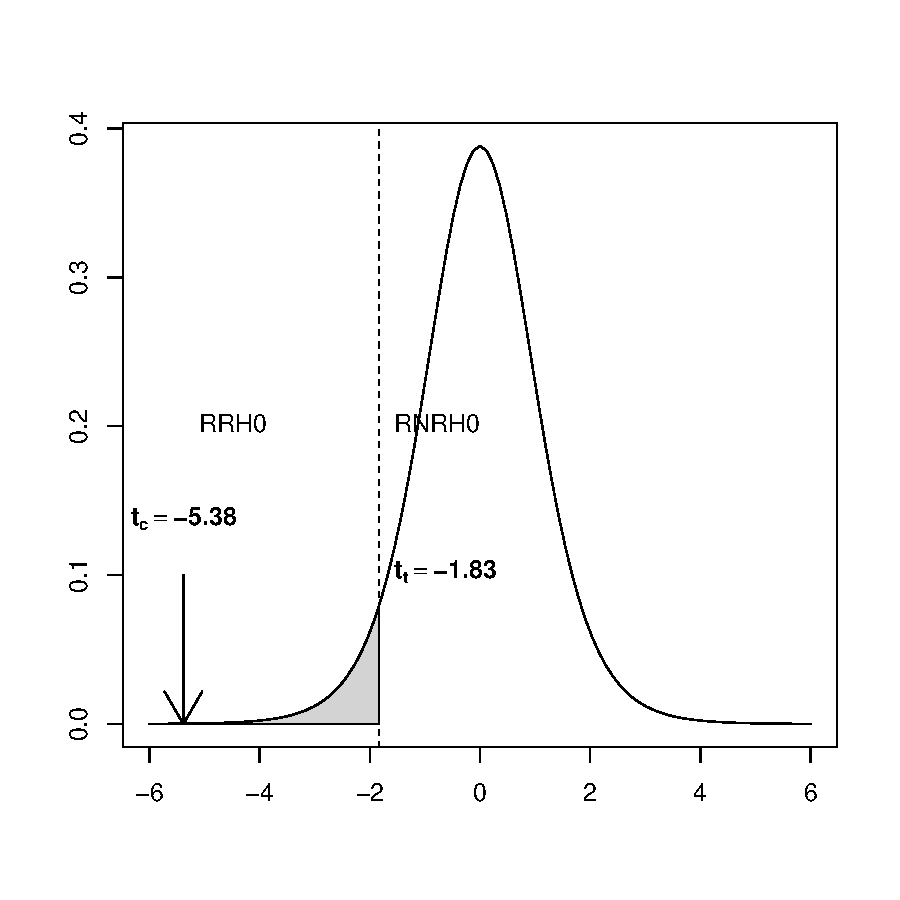
\includegraphics{TH-005}
\end{center}

Decisão: Como $|t_{cal}|>|t_{tab}|$ rejeita-se $H_{0}$ ao nível $\alpha=5\%$ de significância.
%Como $|z_{cal}|>|z_{tab}|$ não rejeita-se $H_{0}$ ao nível $\alpha=AQUI\%$ de significância.
Comandos em R para soluções:

\begin{Schunk}
\begin{Sinput}
> x <- c(34, 41, 36, 41, 29, 32, 38, 35, 33, 30)
> n=length(x)
> df=n-1
> alpha=0.05
> barx <- mean(x)
> dp <- sd(x)
> tt <- qt(alpha,df)
> tc <- (34.9-42)/(4.17/sqrt(10))
> pvalor <- pt(tc,df)
> curve(dt(x,df), from=-6, to=6, xlab="", ylab="")
> polygon(cbind(c(tt,seq(tt,-6, l=100),-6),
+               c(0, dt(seq(tt, -6, l=100),df),
+                 dt(-6,df))),
+         col="lightgray")
> abline(v=tt, lty=2)
> arrows(tc, 0.1, tc, 0)
> tt <- format(tt,digits = 3)
> Tt <- bquote(bold(t[t] == .(tt)))
> tc <- format(tc,digits = 3)
> Tc <- bquote(bold(t[c] == .(tc)))
> text(tt, 0.1, Tt, pos=4)
> text(tt, 0.2, "RNRH0", pos=4)
> text(tc, 0.12, Tc, pos=3)
> text(tc, 0.2, "RRH0", pos=4)
> RR <- "Rejeita-se H0 ao nível de 5% de significância"
> RN <- "Não rejeita-se H0 ao nível de 5% de significância"
> ##Resultado
> ifelse(tc>tt,RR,RN)
\end{Sinput}
\begin{Soutput}
[1] "Rejeita-se H0 ao nível de 5% de significância"
\end{Soutput}
\begin{Sinput}
> ##Ou, equivalentemente:
> ifelse(pvalor > 0.05, RN, RR)
\end{Sinput}
\begin{Soutput}
[1] "Rejeita-se H0 ao nível de 5% de significância"
\end{Soutput}
\begin{Sinput}
> ## estimativa pontual
> (mu.est <- 34.9)
\end{Sinput}
\begin{Soutput}
[1] 34.9
\end{Soutput}
\begin{Sinput}
> ## estimativa intervalar (95%)
> (IC.mu <- mu.est + qt(c(0.025, 0.975),df) * 4.17/sqrt(10))
\end{Sinput}
\begin{Soutput}
[1] 31.91696 37.88304
\end{Soutput}
\end{Schunk}

\item[12.~]O controle de qualidade das peças produzidas por certa fábrica exige que o diâmetro médio das mesmas seja $57$ mm. Para verificar se o processo de produção está sob controle, observam-se os diâmetros de $10$ peças, constatando-se os seguintes valores em mm: $56,5; 56,6; 57,3; 56,9; 57,1; 56,7; 57,1; 56,8; 57,1; 57,0.$ Admitindo-se um nível de significância de $5\%,$ pode-se concluir que o processo de produção está sob controle?

\begin{align*}
H_{0}: \mu&=57mm \\
H_{1}: \mu&\neq 57mm\quad \textrm{(bilateral)}
\end{align*}

Dados:

$n=10;\quad \bar{x}=56.91;\quad S=0.256;\quad \alpha=0.05\% \rightarrow t_{t}=2.262157$

$$t_{cal}=\dfrac{\bar{x}-\mu_{0}}{\dfrac{S}{\sqrt{n}}}=\dfrac{56.91-57}{0.256/\sqrt{10}}=-1.112$$
$$p-valor=0.2947482$$
\begin{center}
\setkeys{Gin}{width=0.5\linewidth}
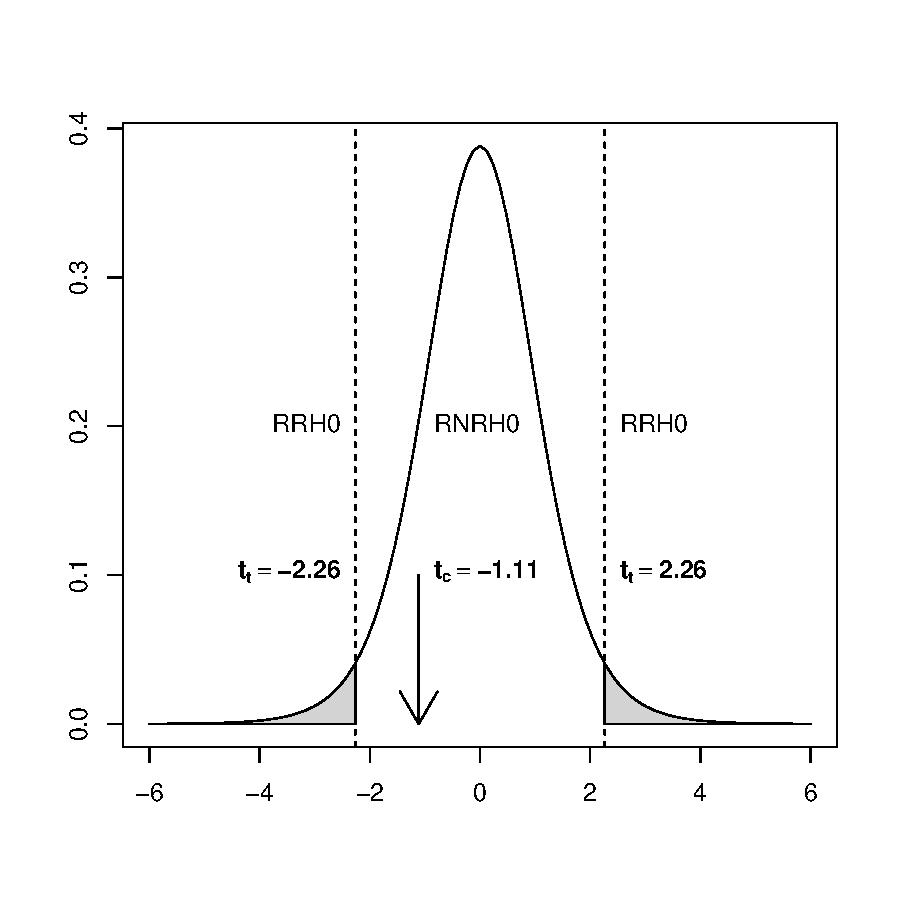
\includegraphics{TH-007}
\end{center}

Decisão: %Como $|t_{cal}|>|t_{tab}|$ rejeita-se $H_{0}$ ao nível $\alpha=AQUI\%$ de significância.
%Como $|z_{cal}|>|z_{tab}|$ não rejeita-se $H_{0}$ ao nível $\alpha=AQUI\%$ de significância.
Comandos em R para soluções:

\begin{Schunk}
\begin{Sinput}
> (x <- c(56.5, 56.6, 57.3, 56.9, 57.1, 56.7, 57.1, 56.8, 57.1, 57.0))
\end{Sinput}
\begin{Soutput}
 [1] 56.5 56.6 57.3 56.9 57.1 56.7 57.1 56.8 57.1 57.0
\end{Soutput}
\begin{Sinput}
> (n=length(x))
\end{Sinput}
\begin{Soutput}
[1] 10
\end{Soutput}
\begin{Sinput}
> (df=n-1)
\end{Sinput}
\begin{Soutput}
[1] 9
\end{Soutput}
\begin{Sinput}
> (alpha=0.025)
\end{Sinput}
\begin{Soutput}
[1] 0.025
\end{Soutput}
\begin{Sinput}
> (barx <- mean(x))
\end{Sinput}
\begin{Soutput}
[1] 56.91
\end{Soutput}
\begin{Sinput}
> (dp <- sd(x))
\end{Sinput}
\begin{Soutput}
[1] 0.2558211
\end{Soutput}
\begin{Sinput}
> (tt <- qt(alpha,df))
\end{Sinput}
\begin{Soutput}
[1] -2.262157
\end{Soutput}
\begin{Sinput}
> (mu <- 57)
\end{Sinput}
\begin{Soutput}
[1] 57
\end{Soutput}
\begin{Sinput}
> (tc <- (barx-mu)/(dp/sqrt(n)))
\end{Sinput}
\begin{Soutput}
[1] -1.112516
\end{Soutput}
\begin{Sinput}
> (pvalor <- 2*pt(tc,df))
\end{Sinput}
\begin{Soutput}
[1] 0.2947482
\end{Soutput}
\begin{Sinput}
> curve(dt(x,df), from=-6, to=6, xlab="", ylab="")
> polygon(cbind(c(-abs(tt),seq(-abs(tt),-6, l=100),-6),
+               c(0, dt(seq(-abs(tt), -6, l=100),df),
+                 dt(-6,df))),
+         col="lightgray")
> polygon(cbind(c(abs(tt),seq(abs(tt),6, l=100),6),
+               c(dt(6,df), dt(seq(abs(tt), 6, l=100),df),
+                 0)),
+         col="lightgray")
> abline(v=tt, lty=2)
> abline(v=-tt, lty=2)
> arrows(tc, 0.1, tc, 0)
> tt1 <- qt(alpha,df)
> tt1 <- format(tt1,digits = 3)
> Tt1 <- bquote(bold(t[t] == .(tt1)))
> tt2 <- -qt(alpha,df)
> tt2 <- format(tt2,digits = 3)
> Tt2 <- bquote(bold(t[t] == .(tt2)))
> tc1 <- format(tc,digits = 3)
> Tc1 <- bquote(bold(t[c] == .(tc1)))
> text(tt1, 0.1, Tt1, pos=2)
> text(tt1, 0.2, "RRH0", pos=2)
> text(tt2, 0.1, Tt2, pos=4)
> text(tt2, 0.2, "RRH0", pos=4)
> text(tc1, 0.1, Tc1, pos=4)
> text(tc1, 0.2, "RNRH0", pos=4)
> RR <- "Rejeita-se H0 ao nível de 5% de significância"
> RN <- "Não rejeita-se H0 ao nível de 5% de significância"
> ##Resultado
> (ifelse((tc<tt || tc>(abs(tt))),RR,RN))
\end{Sinput}
\begin{Soutput}
[1] "Não rejeita-se H0 ao nível de 5% de significância"
\end{Soutput}
\begin{Sinput}
> ##Ou, equivalentemente:
> (ifelse(pvalor > ns, RN, RR))
\end{Sinput}
\begin{Soutput}
[1] "Não rejeita-se H0 ao nível de 5% de significância"
\end{Soutput}
\begin{Sinput}
> ## estimativa pontual
> (mu.est <- barx)
\end{Sinput}
\begin{Soutput}
[1] 56.91
\end{Soutput}
\begin{Sinput}
> ## estimativa intervalar (95%)
> (IC.mu <- mu.est + qt(c((alpha/2), (1-alpha/2)),df) * (dp/sqrt(n)))
\end{Sinput}
\begin{Soutput}
[1] 56.69279 57.12721
\end{Soutput}
\end{Schunk}

\item[13.~]Numa localidade, $32\%$ dos consumidores consomem determinado produto. Foi lançado no mercado da localidade um produto concorrente. Uma pesquisa realizada com 500 consumidores escolhidos ao acaso revelou que 145 dentre estes consomem o antigo produto. Pode-se concluir, num nível de significância de $2\%,$ que a preferência pelo produto antigo diminuiu com a entrada do concorrente no mercado? Calcule o valor da prova para esta amostra.

\begin{align*}
H_{0}: p&=0.32 \\
H_{1}: p&< 0.32\quad \textrm{(unilateral)}
\end{align*}

Dados:

$n=500;\quad \bar{x}=145;\quad p_{0}=0.32;\quad \alpha=2\% \rightarrow z_{t}=-2.054$

$$z_{cal}=\dfrac{\bar{x}-np_{0}}{\sqrt{np_{0}(1-p_{0})}}=\dfrac{145-160}{\sqrt{160(0.68)}}=-1.43$$
$$p-valor=0.07520861$$
\begin{center}
\setkeys{Gin}{width=0.5\linewidth}
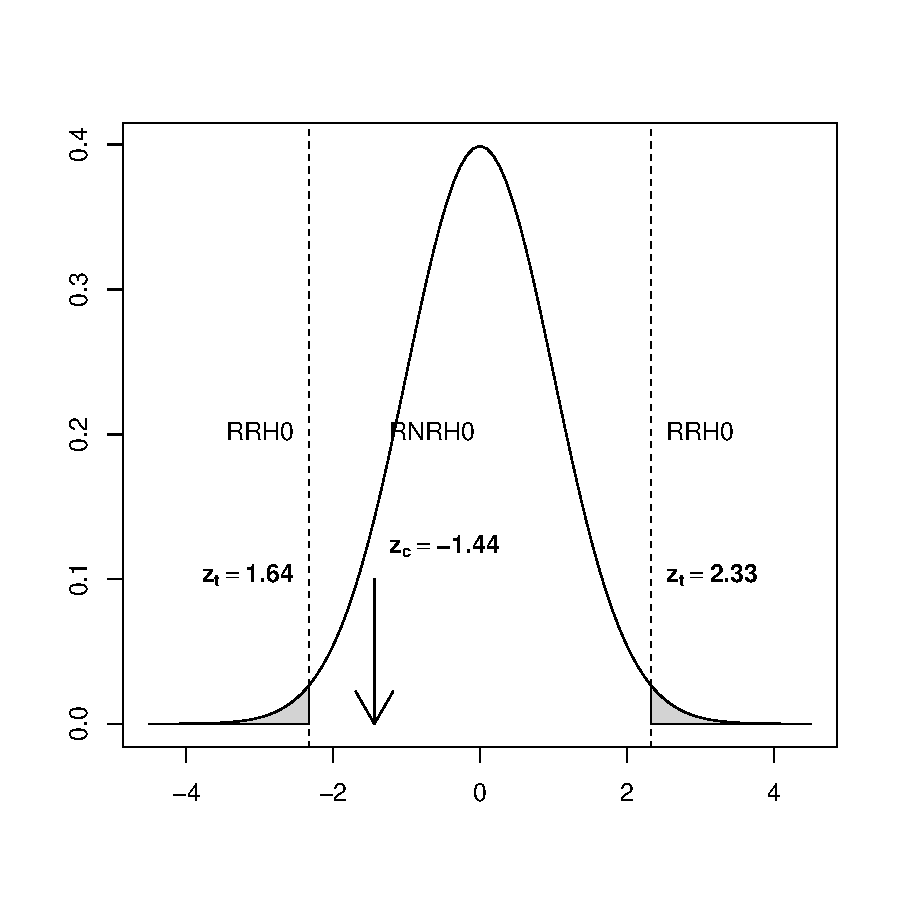
\includegraphics{TH-009}
\end{center}

Decisão: Como %$|z_{cal}|>|z_{tab}|$ rejeita-se $H_{0}$ ao nível $\alpha=AQUI\%$ de significância.
$|z_{cal}|<|z_{tab}|$ não rejeita-se $H_{0}$ ao nível $\alpha=2\%$ de significância.
Comandos em R para soluções:

\begin{Schunk}
\begin{Sinput}
> (ns <- 0.02)
\end{Sinput}
\begin{Soutput}
[1] 0.02
\end{Soutput}
\begin{Sinput}
> (alpha <- 0.02)
\end{Sinput}
\begin{Soutput}
[1] 0.02
\end{Soutput}
\begin{Sinput}
> (n <- 500)
\end{Sinput}
\begin{Soutput}
[1] 500
\end{Soutput}
\begin{Sinput}
> (p0 <- 0.32)
\end{Sinput}
\begin{Soutput}
[1] 0.32
\end{Soutput}
\begin{Sinput}
> (barx <- 145)
\end{Sinput}
\begin{Soutput}
[1] 145
\end{Soutput}
\begin{Sinput}
> (zt <- qnorm(alpha))
\end{Sinput}
\begin{Soutput}
[1] -2.053749
\end{Soutput}
\begin{Sinput}
> (zc <- (barx-(n*p0))/(sqrt(n*p0*(1-p0))))
\end{Sinput}
\begin{Soutput}
[1] -1.438059
\end{Soutput}
\begin{Sinput}
> (pvalor <- pnorm(zc))
\end{Sinput}
\begin{Soutput}
[1] 0.07520861
\end{Soutput}
\begin{Sinput}
> curve(dnorm(x), from=-4.5, to=4.5, xlab="", ylab="")
> polygon(cbind(c(-4.5, seq(-4.5,zt, l=100),zt),
+               c(0, dnorm(seq(-4.5, zt, l=100)),
+                 (0))),
+         col="lightgray")
> abline(v=zt, lty=2)
> arrows(zc, 0.1, zc, 0)
> zt1 <- format(zt,digits = 3)
> Zt1 <- bquote(bold(z[t] == .(zt1)))
> zc1 <- format(zc,digits = 3)
> Zc1 <- bquote(bold(z[c] == .(zc1)))
> text(zt1, 0.1, Zt1, pos=2)
> text(zt1, 0.2, "RRH0", pos=2)
> text(zc1, 0.12, Zc1, pos=4)
> text(zc1, 0.2, "RNRH0", pos=4)
> RR <- "Rejeita-se H0 ao nível de 2% de significância"
> RN <- "Não rejeita-se H0 ao nível de 2% de significância"
> ##Resultado
> ifelse((zc<zt),RR,RN)
\end{Sinput}
\begin{Soutput}
[1] "Não rejeita-se H0 ao nível de 2% de significância"
\end{Soutput}
\begin{Sinput}
> ##Ou, equivalentemente:
> ifelse(pvalor > 0.02, RN, RR)
\end{Sinput}
\begin{Soutput}
[1] "Não rejeita-se H0 ao nível de 2% de significância"
\end{Soutput}
\begin{Sinput}
> ## estimativa pontual
> (mu.est <- 145)
\end{Sinput}
\begin{Soutput}
[1] 145
\end{Soutput}
\begin{Sinput}
> ## estimativa intervalar (98%)
> (IC.mu <- mu.est + qnorm(c(0.02, 0.98)) * (n*p0)/sqrt(n*p0*(1-p0)))
\end{Sinput}
\begin{Soutput}
[1] 113.4969 176.5031
\end{Soutput}
\end{Schunk}

\item[14.~]Sabe-se que $6\%$ das unidades de certo produto são substituídas gratuitamente por apresentar defeitos de fabricação. Para reduzir este percentual, o fabricante investiu na melhoria da qualidade do produto. Consta-se que 12 dentre 400 unidades vendidas tiveram que ser substituídas gratuitamente por apresentar defeitos de fabricação. Pode-se concluir, num nível de significância de $3\%,$ que a qualidade do produto melhorou?

\begin{align*}
H_{0}: p&=0.06 \\
H_{1}: p&< 0.06\quad \textrm{(unilateral)}
\end{align*}

Dados:

$n=400;\quad \bar{x}=12;\quad p_{0}=0.06;\quad \alpha=3\% \rightarrow z_{t}=-1.88$

$$z_{cal}=\dfrac{\bar{x}-np_{0}}{\sqrt{np_{0}(1-p_{0})}}=\dfrac{12-24}{\sqrt{24(0.94)}}=-2.526$$
$$p-valor=0.005760995$$
\begin{center}
\setkeys{Gin}{width=0.5\linewidth}
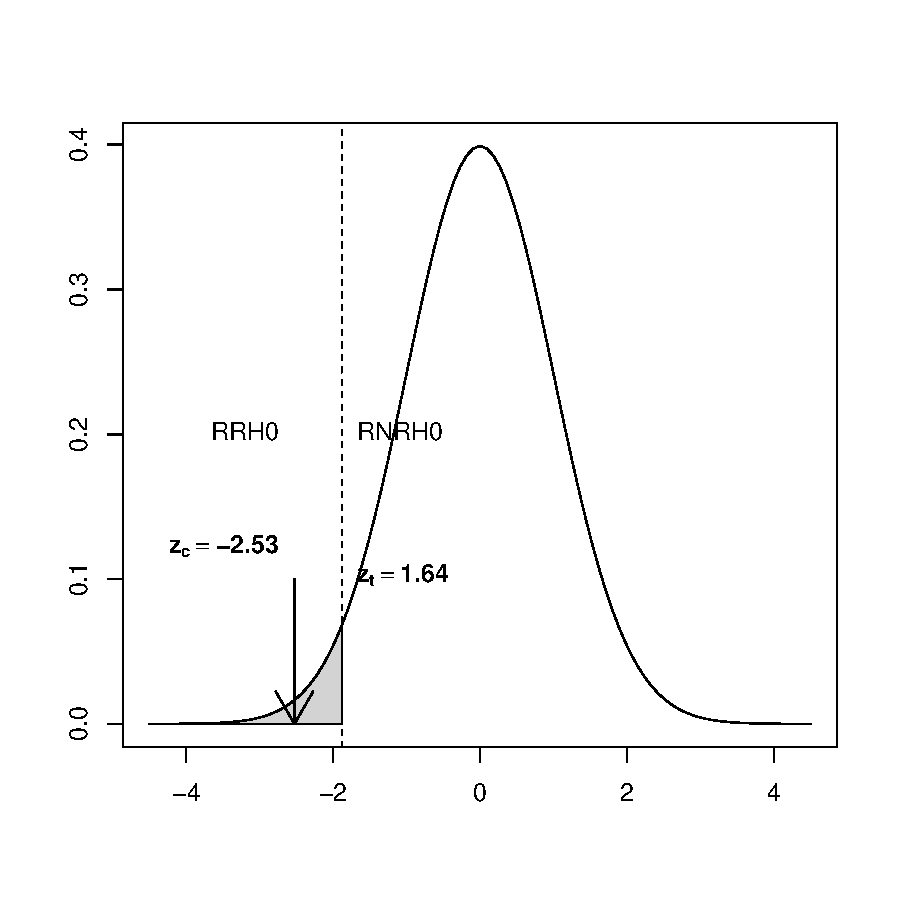
\includegraphics{TH-011}
\end{center}

Decisão: Como $|z_{cal}|>|z_{tab}|$ rejeita-se $H_{0}$ ao nível $\alpha=3\%$ de significância.
%$|z_{cal}|<|z_{tab}|$ não rejeita-se $H_{0}$ ao nível $\alpha=2\%$ de significância.

Comandos em R para soluções:

\begin{Schunk}
\begin{Sinput}
> (alpha <- 0.03)
\end{Sinput}
\begin{Soutput}
[1] 0.03
\end{Soutput}
\begin{Sinput}
> (n <- 400)
\end{Sinput}
\begin{Soutput}
[1] 400
\end{Soutput}
\begin{Sinput}
> (p0 <- 0.06)
\end{Sinput}
\begin{Soutput}
[1] 0.06
\end{Soutput}
\begin{Sinput}
> (barx <- 12)
\end{Sinput}
\begin{Soutput}
[1] 12
\end{Soutput}
\begin{Sinput}
> (zt <- qnorm(alpha))
\end{Sinput}
\begin{Soutput}
[1] -1.880794
\end{Soutput}
\begin{Sinput}
> (zc <- (barx-(n*p0))/(sqrt(n*p0*(1-p0))))
\end{Sinput}
\begin{Soutput}
[1] -2.526456
\end{Soutput}
\begin{Sinput}
> (pvalor <- pnorm(zc))
\end{Sinput}
\begin{Soutput}
[1] 0.005760995
\end{Soutput}
\begin{Sinput}
> curve(dnorm(x), from=-4.5, to=4.5, xlab="", ylab="")
> polygon(cbind(c(-4.5, seq(-4.5,zt, l=100),zt),
+               c(0, dnorm(seq(-4.5, zt, l=100)),
+                 (0))),
+         col="lightgray")
> abline(v=zt, lty=2)
> arrows(zc, 0.1, zc, 0)
> zt1 <- format(zt,digits = 3)
> Zt1 <- bquote(bold(z[t] == .(zt1)))
> zc1 <- format(zc,digits = 3)
> Zc1 <- bquote(bold(z[c] == .(zc1)))
> text(zt1, 0.1, Zt, pos=4)
> text(zt1, 0.2, "RNRH0", pos=4)
> text(zc1, 0.12, Zc1, pos=2)
> text(zc1, 0.2, "RRH0", pos=2)
> RR <- "Rejeita-se H0 ao nível de 3% de significância"
> RN <- "Não rejeita-se H0 ao nível de 3% de significância"
> ##Resultado
> ifelse((zc<zt || zc>abs(zt)),RR,RN)
\end{Sinput}
\begin{Soutput}
[1] "Rejeita-se H0 ao nível de 3% de significância"
\end{Soutput}
\begin{Sinput}
> ##Ou, equivalentemente:
> ifelse(pvalor > 0.03, RN, RR)
\end{Sinput}
\begin{Soutput}
[1] "Rejeita-se H0 ao nível de 3% de significância"
\end{Soutput}
\begin{Sinput}
> ## estimativa pontual
> (mu.est <- 12)
\end{Sinput}
\begin{Soutput}
[1] 12
\end{Soutput}
\begin{Sinput}
> ## estimativa intervalar (98%)
> (IC.mu <- mu.est + qnorm(c(0.015, 0.985)) * (n*p0)/sqrt(n*p0*(1-p0)))
\end{Sinput}
\begin{Soutput}
[1]  1.034725 22.965275
\end{Soutput}
\end{Schunk}

\item[18.~]Uma fábrica de automóveis anuncia que seus carros consomem, em média, 11 litros por 100 km, com desvio padrão de 0,8 litros. Uma revista resolve testar essa afirmação e analisa 35 automóveis dessa marca, obtendo 11,3 litros por 100 km como consumo médio (considerar distribução normal). O que a revista pode concluir sobre o anúncio da fábrica, no nível de $10\%?$

\begin{Schunk}
\begin{Sinput}
> #H0:\mu=0.11km/l
> #H1:\mu!=0.11km/l
> (mu <- 0.11)
\end{Sinput}
\begin{Soutput}
[1] 0.11
\end{Soutput}
\begin{Sinput}
> (sigma <- 0.8)
\end{Sinput}
\begin{Soutput}
[1] 0.8
\end{Soutput}
\begin{Sinput}
> (n <- 35)
\end{Sinput}
\begin{Soutput}
[1] 35
\end{Soutput}
\begin{Sinput}
> (barx <- 0.113)
\end{Sinput}
\begin{Soutput}
[1] 0.113
\end{Soutput}
\begin{Sinput}
> (alpha <- 0.1)
\end{Sinput}
\begin{Soutput}
[1] 0.1
\end{Soutput}
\begin{Sinput}
> (zc <- (barx-mu)/(sigma/sqrt(n)))
\end{Sinput}
\begin{Soutput}
[1] 0.0221853
\end{Soutput}
\begin{Sinput}
> (zt <- qnorm(0.05)) #Teste bilateral
\end{Sinput}
\begin{Soutput}
[1] -1.644854
\end{Soutput}
\begin{Sinput}
> (pvalor <- 2*pnorm(zc))
\end{Sinput}
\begin{Soutput}
[1] 1.0177
\end{Soutput}
\begin{Sinput}
> RR <- "Rejeita-se H0 ao nível de 10% de significância"
> RN <- "Não rejeita-se H0 ao nível de 10% de significância"
> ##Resultado
> ifelse(abs(zc)>abs(zt),RR,RN)
\end{Sinput}
\begin{Soutput}
[1] "Não rejeita-se H0 ao nível de 10% de significância"
\end{Soutput}
\begin{Sinput}
> ##Ou, equivalentemente:
> ifelse(pvalor > 0.1, RN, RR)
\end{Sinput}
\begin{Soutput}
[1] "Não rejeita-se H0 ao nível de 10% de significância"
\end{Soutput}
\end{Schunk}

\item[19.~]Duas máquinas, A e B, são usadas para empacotar pó de café. A experiência passada garante que o desvio padrão para ambas é de 10g. Porém, suspeita-se que elas têm médias diferentes. Para verificar, sortearam-se duas amostras: uma com 25 pacotes da máquina A e outra com 16 pacotes da máquina B. As médias foram, respectivamente, $\bar{x}_{A} = 502,74g$ e $\bar{x}_{B} = 496,60 g$.  Com esses números, e com o nível de $5\%$, qual seria a coclusão do teste $H_0:\mu_A =\mu_B$?

\begin{Schunk}
\begin{Sinput}
> #H0:\muA=\muB
> #H1:\muA!=\muB
> (barxA <- 502.74)
\end{Sinput}
\begin{Soutput}
[1] 502.74
\end{Soutput}
\begin{Sinput}
> (barxB <- 496.60)
\end{Sinput}
\begin{Soutput}
[1] 496.6
\end{Soutput}
\begin{Sinput}
> (sigma <- 10)
\end{Sinput}
\begin{Soutput}
[1] 10
\end{Soutput}
\begin{Sinput}
> (nA <- 25)
\end{Sinput}
\begin{Soutput}
[1] 25
\end{Soutput}
\begin{Sinput}
> (nB <- 16)
\end{Sinput}
\begin{Soutput}
[1] 16
\end{Soutput}
\begin{Sinput}
> (alpha <- 0.05)
\end{Sinput}
\begin{Soutput}
[1] 0.05
\end{Soutput}
\begin{Sinput}
> (zc <- (barxA-barxB)/(sigma*sqrt((1/nA)+(1/nB))))
\end{Sinput}
\begin{Soutput}
[1] 1.917814
\end{Soutput}
\begin{Sinput}
> (zt <- qnorm(0.025)) #Teste bilateral
\end{Sinput}
\begin{Soutput}
[1] -1.959964
\end{Soutput}
\begin{Sinput}
> (pvalor <- 2*pnorm(-zc))
\end{Sinput}
\begin{Soutput}
[1] 0.05513463
\end{Soutput}
\begin{Sinput}
> RR <- "Rejeita-se H0 ao nível de 5% de significância"
> RN <- "Não rejeita-se H0 ao nível de 5% de significância"
> ##Resultado
> ifelse(abs(zc)>abs(zt),RR,RN)
\end{Sinput}
\begin{Soutput}
[1] "Não rejeita-se H0 ao nível de 5% de significância"
\end{Soutput}
\begin{Sinput}
> ##Ou, equivalentemente:
> ifelse(pvalor > 0.05, RN, RR)
\end{Sinput}
\begin{Soutput}
[1] "Não rejeita-se H0 ao nível de 5% de significância"
\end{Soutput}
\end{Schunk}

\item[20.~]Uma fábrica de embalagens para produtos químicos está estudando dois processos para combater a corrosão de suas latas especiais. Para verificar o efeito dos tratamentos, foram usadas amostras cujos resultados estão no quadro abaixo (em porcentagem de corrosão eliminada). Qual seria a conclusão sobre os dois tratamentos?

\begin{tabular}{cccc}\\ \hline
Método & Amostra & Média & Desvio Padrão \\ \hline
A & 15 & 48 & 10 \\
B & 12 & 52 & 15 \\ \hline
\end{tabular}

\begin{Schunk}
\begin{Sinput}
> #H0:\sigma_{A}^{2}=\sigma_{B}^{2}
> #H1:\sigma_{A}^{2}<\sigma_{B}^{2}
> (dpA <- 10)
\end{Sinput}
\begin{Soutput}
[1] 10
\end{Soutput}
\begin{Sinput}
> (dpB <- 15)
\end{Sinput}
\begin{Soutput}
[1] 15
\end{Soutput}
\begin{Sinput}
> (nA <- 15)
\end{Sinput}
\begin{Soutput}
[1] 15
\end{Soutput}
\begin{Sinput}
> (dfA <- nA-1)
\end{Sinput}
\begin{Soutput}
[1] 14
\end{Soutput}
\begin{Sinput}
> (nB <- 12)
\end{Sinput}
\begin{Soutput}
[1] 12
\end{Soutput}
\begin{Sinput}
> (dfB <- nB-1)
\end{Sinput}
\begin{Soutput}
[1] 11
\end{Soutput}
\begin{Sinput}
> (alpha <- 0.05)
\end{Sinput}
\begin{Soutput}
[1] 0.05
\end{Soutput}
\begin{Sinput}
> (fc <- (dpA^2)/(dpB^2))
\end{Sinput}
\begin{Soutput}
[1] 0.4444444
\end{Soutput}
\begin{Sinput}
> (ft <- qf(alpha,dfA,dfB))
\end{Sinput}
\begin{Soutput}
[1] 0.389788
\end{Soutput}
\begin{Sinput}
> (pvalor <-(pf(fc,dfA,dfB)))
\end{Sinput}
\begin{Soutput}
[1] 0.07754768
\end{Soutput}
\begin{Sinput}
> RR <- "Rejeita-se H0 ao nível alpha=5% de significância"
> RN <- "Não rejeita-se H0 ao nível alpha=5% de significância"
> ##Resultado
> ifelse(fc>ft,RN,RR) #Cuidado, aqui temos um teste unilateral a esquerda!
\end{Sinput}
\begin{Soutput}
[1] "Não rejeita-se H0 ao nível alpha=5% de significância"
\end{Soutput}
\begin{Sinput}
> ##Ou, equivalentemente:
> ifelse(pvalor > 0.05, RN, RR) 
\end{Sinput}
\begin{Soutput}
[1] "Não rejeita-se H0 ao nível alpha=5% de significância"
\end{Soutput}
\begin{Sinput}
> #H0:\muA=\muB
> #H1:\muA!=\muB
> (barxA <- 48)
\end{Sinput}
\begin{Soutput}
[1] 48
\end{Soutput}
\begin{Sinput}
> (barxB <- 52)
\end{Sinput}
\begin{Soutput}
[1] 52
\end{Soutput}
\begin{Sinput}
> (nA <- 15)
\end{Sinput}
\begin{Soutput}
[1] 15
\end{Soutput}
\begin{Sinput}
> (nB <- 12)
\end{Sinput}
\begin{Soutput}
[1] 12
\end{Soutput}
\begin{Sinput}
> df <- nA+nB-2
> (Sc2 <- ((nA-1)*(dpA^2)+(nB-1)*(dpB^2))/(nA+nB-2))
\end{Sinput}
\begin{Soutput}
[1] 155
\end{Soutput}
\begin{Sinput}
> (tc <- (barxA-barxB)/(sqrt(Sc2*((1/nA)+(1/nB)))))
\end{Sinput}
\begin{Soutput}
[1] -0.8295614
\end{Soutput}
\begin{Sinput}
> (tt1 <- qt(0.025,df)) #Teste bilateral
\end{Sinput}
\begin{Soutput}
[1] -2.059539
\end{Soutput}
\begin{Sinput}
> (tt2 <- qt(0.975,df)) #Teste bilateral
\end{Sinput}
\begin{Soutput}
[1] 2.059539
\end{Soutput}
\begin{Sinput}
> (pvalor <- 2*(min(pt(tc,df),(1-pt(tc,df)))))
\end{Sinput}
\begin{Soutput}
[1] 0.4146381
\end{Soutput}
\begin{Sinput}
> RR <- "Rejeita-se H0 ao nível de 5% de significância"
> RN <- "Não rejeita-se H0 ao nível de 5% de significância"
> ##Resultado
> ifelse(abs(tc)>abs(tt1),RR,RN)
\end{Sinput}
\begin{Soutput}
[1] "Não rejeita-se H0 ao nível de 5% de significância"
\end{Soutput}
\begin{Sinput}
> ##Ou, equivalentemente:
> ifelse(pvalor > 0.05, RN, RR)
\end{Sinput}
\begin{Soutput}
[1] "Não rejeita-se H0 ao nível de 5% de significância"
\end{Soutput}
\end{Schunk}

\item[21.~]Para investigar a influência da opção profissional sobre o salário inicial de recém-formados, investigaram-se dois grupos de profissionais: um de liberais em geral 
e outro de formandos em Administração de Empresas. Com os resultados abaixo, expressos em salários mínimos, quais seriam suas conclusões?

\begin{tabular}{ccccccccc}\\ \hline
Liberais & 6,6 & 10,3 & 10,8 & 12,9 & 9,2 & 12,3 & 7,0 &  \\ \hline
Administradores & 8,1 & 9,8 & 8,7 & 10,0 & 10,2 & 8,2 & 8,7 & 10,1 \\ \hline
\end{tabular}

\begin{Schunk}
\begin{Sinput}
> #H0:\sigma_{A}^{2}=\sigma_{B}^{2}
> #H1:\sigma_{A}^{2}!=\sigma_{B}^{2}
> (A <- Lib <- c(6.6 , 10.3 , 10.8 , 12.9 , 9.2 , 12.3 , 7.0))
\end{Sinput}
\begin{Soutput}
[1]  6.6 10.3 10.8 12.9  9.2 12.3  7.0
\end{Soutput}
\begin{Sinput}
> (B <- Adm <- c(8.1 , 9.8 , 8.7 , 10.0 , 10.2 , 8.2 , 8.7 , 10.1))
\end{Sinput}
\begin{Soutput}
[1]  8.1  9.8  8.7 10.0 10.2  8.2  8.7 10.1
\end{Soutput}
\begin{Sinput}
> (dpA <- sd(A))
\end{Sinput}
\begin{Soutput}
[1] 2.432909
\end{Soutput}
\begin{Sinput}
> (dpB <- sd(B))
\end{Sinput}
\begin{Soutput}
[1] 0.8876132
\end{Soutput}
\begin{Sinput}
> (nA <- length(A))
\end{Sinput}
\begin{Soutput}
[1] 7
\end{Soutput}
\begin{Sinput}
> (dfA <- nA-1)
\end{Sinput}
\begin{Soutput}
[1] 6
\end{Soutput}
\begin{Sinput}
> (nB <- length(B))
\end{Sinput}
\begin{Soutput}
[1] 8
\end{Soutput}
\begin{Sinput}
> (dfB <- nB-1)
\end{Sinput}
\begin{Soutput}
[1] 7
\end{Soutput}
\begin{Sinput}
> (alpha <- 0.05)
\end{Sinput}
\begin{Soutput}
[1] 0.05
\end{Soutput}
\begin{Sinput}
> (fc <- (dpA^2)/(dpB^2))
\end{Sinput}
\begin{Soutput}
[1] 7.512844
\end{Soutput}
\begin{Sinput}
> (ft1 <- qf(0.025,dfA,dfB, lower.tail=TRUE))
\end{Sinput}
\begin{Soutput}
[1] 0.1755781
\end{Soutput}
\begin{Sinput}
> (ft2 <- qf(0.975,dfA,dfB, lower.tail=TRUE))
\end{Sinput}
\begin{Soutput}
[1] 5.118597
\end{Soutput}
\begin{Sinput}
> (pvalor <-2*pf(fc,dfA,dfB,lower.tail=FALSE))
\end{Sinput}
\begin{Soutput}
[1] 0.01768275
\end{Soutput}
\begin{Sinput}
> (var.test(A,B,alternative = "two.sided"))
\end{Sinput}
\begin{Soutput}
	F test to compare two variances

data:  A and B
F = 7.5128, num df = 6, denom df = 7, p-value = 0.01768
alternative hypothesis: true ratio of variances is not equal to 1
95 percent confidence interval:
  1.467755 42.789180
sample estimates:
ratio of variances 
          7.512844 
\end{Soutput}
\begin{Sinput}
> RR <- "Rejeita-se H0 ao nível alpha=5% de significância"
> RN <- "Não rejeita-se H0 ao nível alpha=5% de significância"
> ##Resultado
> ifelse(fc>ft,RR,RN) #Cuidado, aqui temos um teste unilateral a esquerda!
\end{Sinput}
\begin{Soutput}
[1] "Rejeita-se H0 ao nível alpha=5% de significância"
\end{Soutput}
\begin{Sinput}
> ##Ou, equivalentemente:
> ifelse(pvalor > 0.05, RN, RR) 
\end{Sinput}
\begin{Soutput}
[1] "Rejeita-se H0 ao nível alpha=5% de significância"
\end{Soutput}
\begin{Sinput}
> #H0:\muA=\muB
> #H1:\muA!=\muB
> (barxA <- mean(A))
\end{Sinput}
\begin{Soutput}
[1] 9.871429
\end{Soutput}
\begin{Sinput}
> (barxB <- mean(B))
\end{Sinput}
\begin{Soutput}
[1] 9.225
\end{Soutput}
\begin{Sinput}
> #Variâncias distintas
> (df <- ((((dpA^2)/nA)+((dpB^2)/nB))^2)/(((((dpA^2)/nA)^2)/dfA)+((((dpB^2)/nB)^2)/dfB)))
\end{Sinput}
\begin{Soutput}
[1] 7.393037
\end{Soutput}
\begin{Sinput}
> (tc <- (barxA-barxB)/(sqrt(((dpA^2)/nA)+((dpB^2)/nB))))
\end{Sinput}
\begin{Soutput}
[1] 0.6653048
\end{Soutput}
\begin{Sinput}
> (tt1 <- qt(0.025,df)) #Teste bilateral
\end{Sinput}
\begin{Soutput}
[1] -2.339377
\end{Soutput}
\begin{Sinput}
> (tt2 <- qt(0.975,df)) #Teste bilateral
\end{Sinput}
\begin{Soutput}
[1] 2.339377
\end{Soutput}
\begin{Sinput}
> (pvalor <- 2*(min(pt(tc,df),(1-pt(tc,df)))))
\end{Sinput}
\begin{Soutput}
[1] 0.526061
\end{Soutput}
\begin{Sinput}
> (t.test(A,B,alternative = "two.sided"))
\end{Sinput}
\begin{Soutput}
	Welch Two Sample t-test

data:  A and B
t = 0.6653, df = 7.393, p-value = 0.5261
alternative hypothesis: true difference in means is not equal to 0
95 percent confidence interval:
 -1.626575  2.919433
sample estimates:
mean of x mean of y 
 9.871429  9.225000 
\end{Soutput}
\begin{Sinput}
> RR <- "Rejeita-se H0 ao nível de 5% de significância"
> RN <- "Não rejeita-se H0 ao nível de 5% de significância"
> ##Resultado
> ifelse(abs(tc)>abs(tt),RR,RN)
\end{Sinput}
\begin{Soutput}
[1] "Não rejeita-se H0 ao nível de 5% de significância"
\end{Soutput}
\begin{Sinput}
> ##Ou, equivalentemente:
> ifelse(pvalor > alpha, RN, RR)
\end{Sinput}
\begin{Soutput}
[1] "Não rejeita-se H0 ao nível de 5% de significância"
\end{Soutput}
\end{Schunk}

\item[22.~]Os dados abaixo referem-se a medidas de determinada variável em 19 pessoas antes e depois de uma cirurgia. Verifique se as medidas pré e pós-operatórias 
apresentam a mesma média. Que suposições você faria para resolver o problema?

\begin{tabular}{c|c|c|c|c|c} \hline
 Pessoas  & Pré  & Pós  & Pessoas & Pré  & Pós \\ \hline
 1        & 50,0 & 42,0 & 11      & 50,0 & 48,0      \\
 2        & 50,0 & 42,0 & 12      & 75,0 & 52,0 \\
 3        & 50,0 & 78,0 & 13      & 92,5 & 74,0 \\
 4        & 87,5 & 33,0 & 14      & 38,0 & 47,5 \\
 5        & 32,5 & 96,0 & 15      & 46,5 & 49,0 \\
 6        & 35,0 & 82,0 & 16      & 50,0 & 58,0 \\
 7        & 40,0 & 44,0 & 17      & 30,0 & 42,0 \\
 8        & 45,0 & 31,0 & 18      & 35,0 & 60,0 \\
 9        & 62,5 & 87,0 & 19      & 39,4 & 28,0 \\
 10       & 40,0 & 50,0 & 20      &   -  &  -   \\ \hline
\end{tabular}

\begin{Schunk}
\begin{Sinput}
> (A <- Pre <- c(50.0,50.0,50.0,87.5,32.5,35.0,40.0,45.0,62.5,40.0,50.0,
+                75.0,92.5,38.0,46.5,50.0,30.0,35.0,39.4))
\end{Sinput}
\begin{Soutput}
 [1] 50.0 50.0 50.0 87.5 32.5 35.0 40.0 45.0 62.5 40.0 50.0 75.0 92.5 38.0 46.5
[16] 50.0 30.0 35.0 39.4
\end{Soutput}
\begin{Sinput}
> (B <- Pos <- c(42.0,42.0,78.0,33.0,96.0,82.0,44.0,31.0,87.0,50.0,48.0,
+                52.0,74.0,47.5,49.0,58.0,42.0,60.0,28.0))
\end{Sinput}
\begin{Soutput}
 [1] 42.0 42.0 78.0 33.0 96.0 82.0 44.0 31.0 87.0 50.0 48.0 52.0 74.0 47.5 49.0
[16] 58.0 42.0 60.0 28.0
\end{Soutput}
\begin{Sinput}
> #H0:\muA=\muB (d=\muA-\muB=0)
> #H1:\muA!=\muB (d=\muA-\muB!=0)
> (d <- A-B)
\end{Sinput}
\begin{Soutput}
 [1]   8.0   8.0 -28.0  54.5 -63.5 -47.0  -4.0  14.0 -24.5 -10.0   2.0  23.0
[13]  18.5  -9.5  -2.5  -8.0 -12.0 -25.0  11.4
\end{Soutput}
\begin{Sinput}
> (n <- length(d))
\end{Sinput}
\begin{Soutput}
[1] 19
\end{Soutput}
\begin{Sinput}
> (df <- n-1)
\end{Sinput}
\begin{Soutput}
[1] 18
\end{Soutput}
\begin{Sinput}
> (bard <- mean(d))
\end{Sinput}
\begin{Soutput}
[1] -4.978947
\end{Soutput}
\begin{Sinput}
> (Sd <- sd(d))
\end{Sinput}
\begin{Soutput}
[1] 26.35174
\end{Soutput}
\begin{Sinput}
> (tc <- (bard)/(Sd/sqrt(n)))
\end{Sinput}
\begin{Soutput}
[1] -0.8235787
\end{Soutput}
\begin{Sinput}
> alpha <- 0.05
> (tt1 <- qt(0.025,df)) #Teste bilateral
\end{Sinput}
\begin{Soutput}
[1] -2.100922
\end{Soutput}
\begin{Sinput}
> (tt2 <- qt(0.975,df)) #Teste bilateral
\end{Sinput}
\begin{Soutput}
[1] 2.100922
\end{Soutput}
\begin{Sinput}
> (pvalor <- 2*(min(pt(tc,df),(1-pt(tc,df)))))
\end{Sinput}
\begin{Soutput}
[1] 0.4209576
\end{Soutput}
\begin{Sinput}
> t.test(d,alternative = "two.sided")
\end{Sinput}
\begin{Soutput}
	One Sample t-test

data:  d
t = -0.82358, df = 18, p-value = 0.421
alternative hypothesis: true mean is not equal to 0
95 percent confidence interval:
 -17.680077   7.722183
sample estimates:
mean of x 
-4.978947 
\end{Soutput}
\begin{Sinput}
> RR <- "Rejeita-se H0 ao nível de 5% de significância"
> RN <- "Não rejeita-se H0 ao nível de 5% de significância"
> ##Resultado
> ifelse(abs(tc)>abs(tt),RR,RN)
\end{Sinput}
\begin{Soutput}
[1] "Não rejeita-se H0 ao nível de 5% de significância"
\end{Soutput}
\begin{Sinput}
> ##Ou, equivalentemente:
> ifelse(pvalor > alpha, RN, RR)
\end{Sinput}
\begin{Soutput}
[1] "Não rejeita-se H0 ao nível de 5% de significância"
\end{Soutput}
\end{Schunk}

\item[23~]Uma empresa deseja estudar o efeito de uma pausa de dez minutos para um cafezinho sobre a produtividade de seus trabalhadores. Para isso, sorteou seis operários e contou o número de peças produzidas durante uma semana sem intervalo e uma semana com intervalo. Os resultados sugerem se há ou não melhora na produtividade? 
Caso haja melhora, qual deve ser o acréscimo médio de produção para todos os trabalhadores da fábrica?

\begin{tabular}{ccccccc}\hline
 Operário & 1 & 2 & 3 & 4 & 5 & 6 \\ \hline
 Sem intervalo & 23 & 35 & 29 & 33 & 43 & 32 \\
 Com intervalo & 28 & 38 & 29 & 37 & 42 & 30 \\ \hline
\end{tabular}

\begin{Schunk}
\begin{Sinput}
> (A <- SI <- c(23,35,29,33,43,32))
\end{Sinput}
\begin{Soutput}
[1] 23 35 29 33 43 32
\end{Soutput}
\begin{Sinput}
> (B <- CI <- c(28,38,29,37,42,30))
\end{Sinput}
\begin{Soutput}
[1] 28 38 29 37 42 30
\end{Soutput}
\begin{Sinput}
> #H0: d=0 (d=\muA-\muB=0)
> #H1: d<0 (d=\muA-\muB!=0)
> (d <- SI-CI)
\end{Sinput}
\begin{Soutput}
[1] -5 -3  0 -4  1  2
\end{Soutput}
\begin{Sinput}
> (n <- length(d))
\end{Sinput}
\begin{Soutput}
[1] 6
\end{Soutput}
\begin{Sinput}
> (df <- n-1)
\end{Sinput}
\begin{Soutput}
[1] 5
\end{Soutput}
\begin{Sinput}
> (bard <- mean(d))
\end{Sinput}
\begin{Soutput}
[1] -1.5
\end{Soutput}
\begin{Sinput}
> (Sd <- sd(d))
\end{Sinput}
\begin{Soutput}
[1] 2.880972
\end{Soutput}
\begin{Sinput}
> (tc <- (bard)/(Sd/sqrt(n)))
\end{Sinput}
\begin{Soutput}
[1] -1.275345
\end{Soutput}
\begin{Sinput}
> (alpha <- 0.05)
\end{Sinput}
\begin{Soutput}
[1] 0.05
\end{Soutput}
\begin{Sinput}
> (tt <- qt(0.05,df)) #Teste unilateral
\end{Sinput}
\begin{Soutput}
[1] -2.015048
\end{Soutput}
\begin{Sinput}
> (pvalor <- pt(tc,df))
\end{Sinput}
\begin{Soutput}
[1] 0.129114
\end{Soutput}
\begin{Sinput}
> t.test(d,alternative = "less")
\end{Sinput}
\begin{Soutput}
	One Sample t-test

data:  d
t = -1.2753, df = 5, p-value = 0.1291
alternative hypothesis: true mean is less than 0
95 percent confidence interval:
     -Inf 0.870003
sample estimates:
mean of x 
     -1.5 
\end{Soutput}
\begin{Sinput}
> RR <- "Rejeita-se H0 ao nível de 5% de significância"
> RN <- "Não rejeita-se H0 ao nível de 5% de significância"
> ##Resultado
> ifelse(abs(tc)>abs(tt),RR,RN)
\end{Sinput}
\begin{Soutput}
[1] "Não rejeita-se H0 ao nível de 5% de significância"
\end{Soutput}
\begin{Sinput}
> ##Ou, equivalentemente:
> ifelse(pvalor > alpha, RN, RR)
\end{Sinput}
\begin{Soutput}
[1] "Não rejeita-se H0 ao nível de 5% de significância"
\end{Soutput}
\end{Schunk}

\item[24~] Num levantamento feito com os operários da indústria mecânica, chegou-se aos seguintes números: salário médio $= 3,64$ salários mínimos e desvio padrão $= 0,85$ 
salário mínimo. Suspeita-se que os salários de subclasse formada pelos torneiros mecânicos são diferentes dos salários do conjunto todo, tanto na média como na variância. Que conclusões você obteria se uma amostra de 25 torneiros apresentasse salário médio igual a $4,22$ salários mínimos e desvio padrão igual a $1,25$ salário mínimo?

\begin{Schunk}
\begin{Sinput}
> #H0: \sigma =0.85
> #H1: \sigma!=0.85
> (barx=4.22)
\end{Sinput}
\begin{Soutput}
[1] 4.22
\end{Soutput}
\begin{Sinput}
> (S=1.25)
\end{Sinput}
\begin{Soutput}
[1] 1.25
\end{Soutput}
\begin{Sinput}
> (sigma=0.85)
\end{Sinput}
\begin{Soutput}
[1] 0.85
\end{Soutput}
\begin{Sinput}
> (n <- 25)
\end{Sinput}
\begin{Soutput}
[1] 25
\end{Soutput}
\begin{Sinput}
> (df <- n-1)
\end{Sinput}
\begin{Soutput}
[1] 24
\end{Soutput}
\begin{Sinput}
> (alpha=0.05)
\end{Sinput}
\begin{Soutput}
[1] 0.05
\end{Soutput}
\begin{Sinput}
> (qui_c <- ((n-1)*S^2)/(sigma^2))
\end{Sinput}
\begin{Soutput}
[1] 51.90311
\end{Soutput}
\begin{Sinput}
> (pvalor <- 2*pchisq((alpha/2),(n-1)))
\end{Sinput}
\begin{Soutput}
[1] 6.006234e-32
\end{Soutput}
\begin{Sinput}
> (qui_t1 <- qchisq((alpha/2),(n-1),lower.tail = TRUE))
\end{Sinput}
\begin{Soutput}
[1] 12.40115
\end{Soutput}
\begin{Sinput}
> (qui_t2 <- qchisq((1-(alpha/2)),(n-1),lower.tail = TRUE))
\end{Sinput}
\begin{Soutput}
[1] 39.36408
\end{Soutput}
\begin{Sinput}
> RR <- "Rejeita-se H0 ao nível de 5% de significância"
> RN <- "Não rejeita-se H0 ao nível de 5% de significância"
> ##Resultado
> ifelse((qui_c<qui_t1 || qui_c>qui_t2),RR,RN)
\end{Sinput}
\begin{Soutput}
[1] "Rejeita-se H0 ao nível de 5% de significância"
\end{Soutput}
\begin{Sinput}
> ##Ou, equivalentemente:
> ifelse(pvalor > alpha, RN, RR)
\end{Sinput}
\begin{Soutput}
[1] "Rejeita-se H0 ao nível de 5% de significância"
\end{Soutput}
\begin{Sinput}
> #Como, pelo teste qui-quadrado, a variância populacional é diferente da variância 
> #do levantamento, faremos um teste t para média, supondo variância populacional #desconhecida 
> #H0: \mu =3.64
> #H1: \mu!=3.64
> mu <- 3.64
> (tc <- (barx-mu)/(S/sqrt(n)))
\end{Sinput}
\begin{Soutput}
[1] 2.32
\end{Soutput}
\begin{Sinput}
> (tt1 <- qt(0.025,df,lower.tail = TRUE)) #Teste bilateral
\end{Sinput}
\begin{Soutput}
[1] -2.063899
\end{Soutput}
\begin{Sinput}
> (tt2 <- qt(0.975,df,lower.tail = TRUE)) #Teste bilateral
\end{Sinput}
\begin{Soutput}
[1] 2.063899
\end{Soutput}
\begin{Sinput}
> (pvalor <- 2*(min(pt(tc,df),(1-pt(tc,df)))))
\end{Sinput}
\begin{Soutput}
[1] 0.02916553
\end{Soutput}
\begin{Sinput}
> RR <- "Rejeita-se H0 ao nível de 5% de significância"
> RN <- "Não rejeita-se H0 ao nível de 5% de significância"
> ##Resultado
> ifelse(abs(tc)>abs(tt1),RR,RN)
\end{Sinput}
\begin{Soutput}
[1] "Rejeita-se H0 ao nível de 5% de significância"
\end{Soutput}
\begin{Sinput}
> ##Ou, equivalentemente:
> ifelse(pvalor > alpha, RN, RR)
\end{Sinput}
\begin{Soutput}
[1] "Rejeita-se H0 ao nível de 5% de significância"
\end{Soutput}
\begin{Sinput}
> #Logo, o salário médio dos torneiros mecânicos é diferente do salário médio dos operários!
\end{Sinput}
\end{Schunk}

\item[26~] Um partido afirma que a porcentagem de votos masculinos a seu favor será de $10\%$ a mais do que a porcentagem de votos femininos. Numa pesquisa feita entre 
400 homens, 170 votariam no partido, enquanto entre 625 mulheres, 194 lhe seriam favoráveis. A afirmação do partido é verdadeira ou não?

\begin{Schunk}
\begin{Sinput}
> #H0: pH-pM=0.10
> #H1: pH-pM>0.10
> (p <- 0.10)
\end{Sinput}
\begin{Soutput}
[1] 0.1
\end{Soutput}
\begin{Sinput}
> (pH_est <- 170/400)
\end{Sinput}
\begin{Soutput}
[1] 0.425
\end{Soutput}
\begin{Sinput}
> (nH <- 400)
\end{Sinput}
\begin{Soutput}
[1] 400
\end{Soutput}
\begin{Sinput}
> (pM_est <- 194/625)
\end{Sinput}
\begin{Soutput}
[1] 0.3104
\end{Soutput}
\begin{Sinput}
> (nM <- 625)
\end{Sinput}
\begin{Soutput}
[1] 625
\end{Soutput}
\begin{Sinput}
> (alpha <- 0.05)
\end{Sinput}
\begin{Soutput}
[1] 0.05
\end{Soutput}
\begin{Sinput}
> (zc <- ((pH_est-pM_est)-(p))/sqrt(((pH_est*(1-pH_est))/nH)+((pM_est*(1-pM_est))/nM)))
\end{Sinput}
\begin{Soutput}
[1] 0.4728361
\end{Soutput}
\begin{Sinput}
> (zt <- qnorm(1-alpha))
\end{Sinput}
\begin{Soutput}
[1] 1.644854
\end{Soutput}
\begin{Sinput}
> (pvalor <- pnorm(alpha,lower.tail = FALSE))
\end{Sinput}
\begin{Soutput}
[1] 0.4800612
\end{Soutput}
\begin{Sinput}
> RR <- "Rejeita-se H0 ao nível de 5% de significância"
> RN <- "Não rejeita-se H0 ao nível de 5% de significância"
> ##Resultado
> ifelse((zc>zt),RR,RN)
\end{Sinput}
\begin{Soutput}
[1] "Não rejeita-se H0 ao nível de 5% de significância"
\end{Soutput}
\begin{Sinput}
> ##Ou, equivalentemente:
> ifelse(pvalor > alpha, RN, RR)
\end{Sinput}
\begin{Soutput}
[1] "Não rejeita-se H0 ao nível de 5% de significância"
\end{Soutput}
\end{Schunk}

\item[27~] De 400 moradores sorteados de uma grande cidade industrial, 300 são  favoráveis a um projeto governamental, e de uma amostra de 160 moradores de uma cidade 
cuja principal atividade é o turismo, 120 são contra.
\begin{tasks}
\task Você diria que a diferença de opiniões nas duas cidades é estatisticamente significante? Sim, ver resultados abaixo:
\end{tasks}

\begin{Schunk}
\begin{Sinput}
> #H0: pI=pT
> #H1: pI!=pT
> (p <- 0)
\end{Sinput}
\begin{Soutput}
[1] 0
\end{Soutput}
\begin{Sinput}
> (pI_est <- 300/400)
\end{Sinput}
\begin{Soutput}
[1] 0.75
\end{Soutput}
\begin{Sinput}
> (nI <- 400)
\end{Sinput}
\begin{Soutput}
[1] 400
\end{Soutput}
\begin{Sinput}
> (pT_est <- 40/160)
\end{Sinput}
\begin{Soutput}
[1] 0.25
\end{Soutput}
\begin{Sinput}
> (nT <- 160)
\end{Sinput}
\begin{Soutput}
[1] 160
\end{Soutput}
\begin{Sinput}
> (alpha <- 0.05)
\end{Sinput}
\begin{Soutput}
[1] 0.05
\end{Soutput}
\begin{Sinput}
> (zc <- ((pI_est-pT_est)-(p))/sqrt(((pI_est*(1-pI_est))/nI)+((pT_est*(1-pT_est))/nT)))
\end{Sinput}
\begin{Soutput}
[1] 12.34427
\end{Soutput}
\begin{Sinput}
> (zt1 <- qnorm((alpha/2),lower.tail = TRUE))
\end{Sinput}
\begin{Soutput}
[1] -1.959964
\end{Soutput}
\begin{Sinput}
> (zt2 <- qnorm(1-(alpha/2),lower.tail = TRUE))
\end{Sinput}
\begin{Soutput}
[1] 1.959964
\end{Soutput}
\begin{Sinput}
> (pvalor <- 2*min(pnorm(zc),1-pnorm(zc)))
\end{Sinput}
\begin{Soutput}
[1] 0
\end{Soutput}
\begin{Sinput}
> RR <- "Rejeita-se H0 ao nível de 5% de significância"
> RN <- "Não rejeita-se H0 ao nível de 5% de significância"
> ##Resultado
> ifelse((zc>zt),RR,RN)
\end{Sinput}
\begin{Soutput}
[1] "Rejeita-se H0 ao nível de 5% de significância"
\end{Soutput}
\begin{Sinput}
> ##Ou, equivalentemente:
> ifelse(pvalor > alpha, RN, RR)
\end{Sinput}
\begin{Soutput}
[1] "Rejeita-se H0 ao nível de 5% de significância"
\end{Soutput}
\end{Schunk}

\item[28~] Para verificar o grau de adesão de uma nova cola para vidros, preparam-se dois tipos de montagem: cruzado (A), onde a cola é posta em forma de X, e quadrado (B), onde a cola é posta apenas nas quatro bordas. Os resultados da resistência para as duas amostras de 10 cada estão abaixo. Que tipo de conclusão poderia ser tirada?

\begin{tabular}{c|c|c|c|c|c|c|c|c|c|c} \hline
Método A & 16 & 14 & 19 & 18 & 19 & 20 & 15 & 18 & 17 & 18 \\ \hline
Método B & 13 & 19 & 14 & 17 & 21 & 24 & 10 & 14 & 13 & 15 \\ \hline
\end{tabular}

\begin{Schunk}
\begin{Sinput}
> #H0: sigma_{A}^{2} =sigma_{B}^{2}
> #H1: sigma_{A}^{2} !=sigma_{B}^{2}
> (A <- c(16,14,19,18,19,20,15,18,17,18))
\end{Sinput}
\begin{Soutput}
 [1] 16 14 19 18 19 20 15 18 17 18
\end{Soutput}
\begin{Sinput}
> (B <- c(13,19,14,17,21,24,10,14,13,15))
\end{Sinput}
\begin{Soutput}
 [1] 13 19 14 17 21 24 10 14 13 15
\end{Soutput}
\begin{Sinput}
> (dpA <- sd(A))
\end{Sinput}
\begin{Soutput}
[1] 1.897367
\end{Soutput}
\begin{Sinput}
> (nA <- length(A))
\end{Sinput}
\begin{Soutput}
[1] 10
\end{Soutput}
\begin{Sinput}
> (dfA <- nA-1)
\end{Sinput}
\begin{Soutput}
[1] 9
\end{Soutput}
\begin{Sinput}
> (dpB <- sd(B))
\end{Sinput}
\begin{Soutput}
[1] 4.242641
\end{Soutput}
\begin{Sinput}
> (nB <- length(B))
\end{Sinput}
\begin{Soutput}
[1] 10
\end{Soutput}
\begin{Sinput}
> (dfB <- nB-1)
\end{Sinput}
\begin{Soutput}
[1] 9
\end{Soutput}
\begin{Sinput}
> (alpha <- 0.05)
\end{Sinput}
\begin{Soutput}
[1] 0.05
\end{Soutput}
\begin{Sinput}
> (fc <- (dpA^2)/(dpB^2))
\end{Sinput}
\begin{Soutput}
[1] 0.2
\end{Soutput}
\begin{Sinput}
> (ft1 <- qf((alpha/2),dfA,dfB,lower.tail = TRUE))
\end{Sinput}
\begin{Soutput}
[1] 0.2483859
\end{Soutput}
\begin{Sinput}
> (ft2 <- qf(1-(alpha/2),dfA,dfB,lower.tail = TRUE))
\end{Sinput}
\begin{Soutput}
[1] 4.025994
\end{Soutput}
\begin{Sinput}
> (pvalor <- 2*min(pf(fc,dfA,dfB,lower.tail = TRUE),1-pf(fc,dfA,dfB,lower.tail = TRUE)))
\end{Sinput}
\begin{Soutput}
[1] 0.02507092
\end{Soutput}
\begin{Sinput}
> (var.test(A,B,alternative = "two.sided"))
\end{Sinput}
\begin{Soutput}
	F test to compare two variances

data:  A and B
F = 0.2, num df = 9, denom df = 9, p-value = 0.02507
alternative hypothesis: true ratio of variances is not equal to 1
95 percent confidence interval:
 0.04967717 0.80519883
sample estimates:
ratio of variances 
               0.2 
\end{Soutput}
\begin{Sinput}
> RR <- "Rejeita-se H0 ao nível de 5% de significância"
> RN <- "Não rejeita-se H0 ao nível de 5% de significância"
> ##Resultado
> ifelse((fc<ft1 || fc>ft2),RR,RN)
\end{Sinput}
\begin{Soutput}
[1] "Rejeita-se H0 ao nível de 5% de significância"
\end{Soutput}
\begin{Sinput}
> ##Ou, equivalentemente:
> ifelse(pvalor > alpha, RN, RR)
\end{Sinput}
\begin{Soutput}
[1] "Rejeita-se H0 ao nível de 5% de significância"
\end{Soutput}
\begin{Sinput}
> #H0: muA =muB
> #H1: muA>muB
> (barA <- mean(A))
\end{Sinput}
\begin{Soutput}
[1] 17.4
\end{Soutput}
\begin{Sinput}
> (barB <- mean(B))
\end{Sinput}
\begin{Soutput}
[1] 16
\end{Soutput}
\begin{Sinput}
> (df <- ((((dpA^2)/nA)+((dpB^2)/nB))^2)/(((((dpA^2)/nA)^2)/dfA)+((((dpB^2)/nB)^2)/dfB)))
\end{Sinput}
\begin{Soutput}
[1] 12.46154
\end{Soutput}
\begin{Sinput}
> (tc <- (barA-barB)/(sqrt(((dpA^2)/nA)+((dpB^2)/nB))))
\end{Sinput}
\begin{Soutput}
[1] 0.9525793
\end{Soutput}
\begin{Sinput}
> (tt <- qt(1-alpha,df,lower.tail = TRUE))
\end{Sinput}
\begin{Soutput}
[1] 1.776804
\end{Soutput}
\begin{Sinput}
> (pvalor <- pt(tc,df,lower.tail = FALSE))
\end{Sinput}
\begin{Soutput}
[1] 0.1794578
\end{Soutput}
\begin{Sinput}
> (t.test(A,B,alternative = "greater"))
\end{Sinput}
\begin{Soutput}
	Welch Two Sample t-test

data:  A and B
t = 0.95258, df = 12.462, p-value = 0.1795
alternative hypothesis: true difference in means is greater than 0
95 percent confidence interval:
 -1.211357       Inf
sample estimates:
mean of x mean of y 
     17.4      16.0 
\end{Soutput}
\begin{Sinput}
> RR <- "Rejeita-se H0 ao nível de 5% de significância"
> RN <- "Não rejeita-se H0 ao nível de 5% de significância"
> ##Resultado
> ifelse((tc>tt),RR,RN)
\end{Sinput}
\begin{Soutput}
[1] "Não rejeita-se H0 ao nível de 5% de significância"
\end{Soutput}
\begin{Sinput}
> ##Ou, equivalentemente:
> ifelse(pvalor > alpha, RN, RR)
\end{Sinput}
\begin{Soutput}
[1] "Não rejeita-se H0 ao nível de 5% de significância"
\end{Soutput}
\end{Schunk}

\item[29~] Em um estudo para comparar os efeitos de duas dietas, A e B, sobre o crescimento, 6 ratos foram submetidos à dieta A, e 9 ratos à dieta B. Após 5 semanas, os ganhos em peso foram:

\begin{tabular}{c|c|c|c|c|c|c|c|c|c} \hline
Dieta A & 15 & 18 & 12 & 11 & 14 & 15 &  & &  \\ \hline
Dieta B & 11 & 11 & 12 & 16 & 12 & 13 & 8 & 10 & 13  \\ \hline
\end{tabular}
\begin{tasks}
\task Admitindo que temos duas amostras independentes de populações normais, teste a hipótese de que não há diferença entre as duas dietas, contra a alternativa que a 
dieta A é mais eficaz, usando o teste $t$ de Student, no nível de $\alpha = 0,01$.
\end{tasks}

\begin{Schunk}
\begin{Sinput}
> #H0: sigma_{A}^{2} =sigma_{B}^{2}
> #H1: sigma_{A}^{2} !=sigma_{B}^{2}
> (A <- c(15,18,12,11,14,15))
\end{Sinput}
\begin{Soutput}
[1] 15 18 12 11 14 15
\end{Soutput}
\begin{Sinput}
> (B <- c(11,11,12,16,12,13,8,10,13))
\end{Sinput}
\begin{Soutput}
[1] 11 11 12 16 12 13  8 10 13
\end{Soutput}
\begin{Sinput}
> (dpA <- sd(A))
\end{Sinput}
\begin{Soutput}
[1] 2.483277
\end{Soutput}
\begin{Sinput}
> (nA <- length(A))
\end{Sinput}
\begin{Soutput}
[1] 6
\end{Soutput}
\begin{Sinput}
> (dfA <- nA-1)
\end{Sinput}
\begin{Soutput}
[1] 5
\end{Soutput}
\begin{Sinput}
> (dpB <- sd(B))
\end{Sinput}
\begin{Soutput}
[1] 2.223611
\end{Soutput}
\begin{Sinput}
> (nB <- length(B))
\end{Sinput}
\begin{Soutput}
[1] 9
\end{Soutput}
\begin{Sinput}
> (dfB <- nB-1)
\end{Sinput}
\begin{Soutput}
[1] 8
\end{Soutput}
\begin{Sinput}
> (alpha <- 0.01)
\end{Sinput}
\begin{Soutput}
[1] 0.01
\end{Soutput}
\begin{Sinput}
> (fc <- (dpA^2)/(dpB^2))
\end{Sinput}
\begin{Soutput}
[1] 1.247191
\end{Soutput}
\begin{Sinput}
> (ft1 <- qf((alpha/2),dfA,dfB,lower.tail = TRUE))
\end{Sinput}
\begin{Soutput}
[1] 0.0716283
\end{Soutput}
\begin{Sinput}
> (ft2 <- qf(1-(alpha/2),dfA,dfB,lower.tail = TRUE))
\end{Sinput}
\begin{Soutput}
[1] 8.301799
\end{Soutput}
\begin{Sinput}
> (pvalor <- 2*min(pf(fc,dfA,dfB,lower.tail = TRUE),1-pf(fc,dfA,dfB,lower.tail = TRUE)))
\end{Sinput}
\begin{Soutput}
[1] 0.7424555
\end{Soutput}
\begin{Sinput}
> (var.test(A,B,alternative = "two.sided"))
\end{Sinput}
\begin{Soutput}
	F test to compare two variances

data:  A and B
F = 1.2472, num df = 5, denom df = 8, p-value = 0.7425
alternative hypothesis: true ratio of variances is not equal to 1
95 percent confidence interval:
 0.2588997 8.4274842
sample estimates:
ratio of variances 
          1.247191 
\end{Soutput}
\begin{Sinput}
> RR <- "Rejeita-se H0 ao nível de 5% de significância"
> RN <- "Não rejeita-se H0 ao nível de 5% de significância"
> ##Resultado
> ifelse((fc<ft1 || fc>ft2),RR,RN)
\end{Sinput}
\begin{Soutput}
[1] "Não rejeita-se H0 ao nível de 5% de significância"
\end{Soutput}
\begin{Sinput}
> ##Ou, equivalentemente:
> ifelse(pvalor > alpha, RN, RR)
\end{Sinput}
\begin{Soutput}
[1] "Não rejeita-se H0 ao nível de 5% de significância"
\end{Soutput}
\begin{Sinput}
> #H0: muA =muB
> #H1: muA!=muB
> (barA <- mean(A))
\end{Sinput}
\begin{Soutput}
[1] 14.16667
\end{Soutput}
\begin{Sinput}
> (barB <- mean(B))
\end{Sinput}
\begin{Soutput}
[1] 11.77778
\end{Soutput}
\begin{Sinput}
> (df <- dfA+dfB)
\end{Sinput}
\begin{Soutput}
[1] 13
\end{Soutput}
\begin{Sinput}
> (Sc2 <- (dfA*dpA^2+dfB*dpB^2)/df)
\end{Sinput}
\begin{Soutput}
[1] 5.41453
\end{Soutput}
\begin{Sinput}
> (tc <- (barA-barB)/(sqrt(Sc2*(1/nA+1/nB))))
\end{Sinput}
\begin{Soutput}
[1] 1.947901
\end{Soutput}
\begin{Sinput}
> (tt1 <- qt(alpha/2,df,lower.tail = TRUE))
\end{Sinput}
\begin{Soutput}
[1] -3.012276
\end{Soutput}
\begin{Sinput}
> (tt2 <- qt(1-alpha/2,df,lower.tail = TRUE))
\end{Sinput}
\begin{Soutput}
[1] 3.012276
\end{Soutput}
\begin{Sinput}
> (pvalor <- 2*min(pt(tc,df,lower.tail = TRUE),1-pt(tc,df,lower.tail = TRUE)))
\end{Sinput}
\begin{Soutput}
[1] 0.07335015
\end{Soutput}
\begin{Sinput}
> (t.test(A,B,alternative = "two.sided",var.equal = TRUE))
\end{Sinput}
\begin{Soutput}
	Two Sample t-test

data:  A and B
t = 1.9479, df = 13, p-value = 0.07335
alternative hypothesis: true difference in means is not equal to 0
95 percent confidence interval:
 -0.2605688  5.0383466
sample estimates:
mean of x mean of y 
 14.16667  11.77778 
\end{Soutput}
\begin{Sinput}
> RR <- "Rejeita-se H0 ao nível de 5% de significância"
> RN <- "Não rejeita-se H0 ao nível de 5% de significância"
> ##Resultado
> ifelse((tc<tt1||tc>tt2),RR,RN)
\end{Sinput}
\begin{Soutput}
[1] "Não rejeita-se H0 ao nível de 5% de significância"
\end{Soutput}
\begin{Sinput}
> ##Ou, equivalentemente:
> ifelse(pvalor > alpha, RN, RR)
\end{Sinput}
\begin{Soutput}
[1] "Não rejeita-se H0 ao nível de 5% de significância"
\end{Soutput}
\end{Schunk}

\end{ManualExercise}
\end{Exercise}

\end{document}
